\documentclass{amsart}
\usepackage{graphicx}
\graphicspath{{./}}
\usepackage{hyperref}
\usepackage{csvsimple}
\usepackage{longtable}
\usepackage{epigraph}
\title{Moral Value Distribution of Bad People}
\author{Zulfikar Moinuddin Ahmed}
\date{\today}
\begin{document}
\maketitle

\section{Graphical Representation of Moral Values of Bad People}

I took those people whose answers to "political violence is justified" is 9 or 10 out of 10, very strong support.  I discovered that they are bad people in moral values.

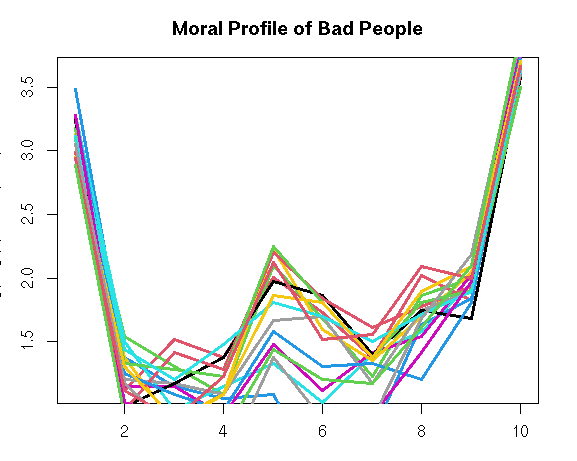
\includegraphics[scale=0.8]{bad.jpeg}

These are conditional distributions of Q177--Q195, various moral values in 1--10 in World Values Surveys, conditioned on $Q192=9$ or $Q192=10$.

\section{Importance of Discovery and My Priority}

In the entire history of Homo Sapiens, no one had discovered the issues of Human Nature more clearly than this graph above.  These are empirical measurements of people around the world of all ethnicities.  They are models for moral values of universal bad people, and across the various different moral issues, we see remarkable uniformity.  These are highly non-trivial analytically.  I had to work very hard to understand the Rousseau exponential on the left and the Hobbes Exponential on the right.  

Now we are in a position to attempt to understand the elements in the middle which are mysterious.  The uniformity of the features is clear, but we do not have a scientific model for them yet.  

I am extremely concerned that credit for this profound discovery, which is work of the greatest genius as well of felicity of serendipity and fortune, might be claimed by others.  This discovery is one of the most profound not just in the history of science, which is not even four centuries old, from Descartes' {\em Meditations}, 1641, but for the history of all of Human Civilisation, which goes back seven thousand odd years to Mesopotamia, today's Iraq and Syria.  No one had any discovery in this entire period that could elucidate clearly the moral nature of Man and the speculations surrounding it from Ancient philosophers in East and West to David Hume, Adam Smith, Immanuel Kant of the Enlightenment period have been without sufficient care for measurement and analytical models.  I am the first man in history of Human Race to have provided any analytical models at all.

We are today standing on the threshold of one of the great transitions of Human Civilisation that will rival the Ancient Greek Birth of Tragedy for the first time.

\end{document}